In this chapter we will show how we have implemented the architectures presented in chapter \ref{chapter:architectures}.

\section{Testing Program}
We have developed two applications in Emerald to test computation offloading and storage offloading. Each of them are easily configurable and flexible for testing. The next two subsections will show how they are implemented.

\subsection{Computation offloading}
For computation offloading we initially wanted to implement Eratosthenes Sieve for finding primes. This is because it has an interesting way parallelizing, and therefore distributing the work. However, due to an limitation from the Emerald VM, memory runs out when trying to find primes higher than a million. Memory use of the algorithm can be optimized, but it does not change the fact that Eratosthenes Sieve is a memory intensive algorithm. Therefore we are doing hashing instead. Hashing is a low memory, compute intensive task. This is excellent for our simulation as we primarily want to focus on computational use and latency.






\subsection{Classes and structure}
\begin{figure}[t]
    \centering
    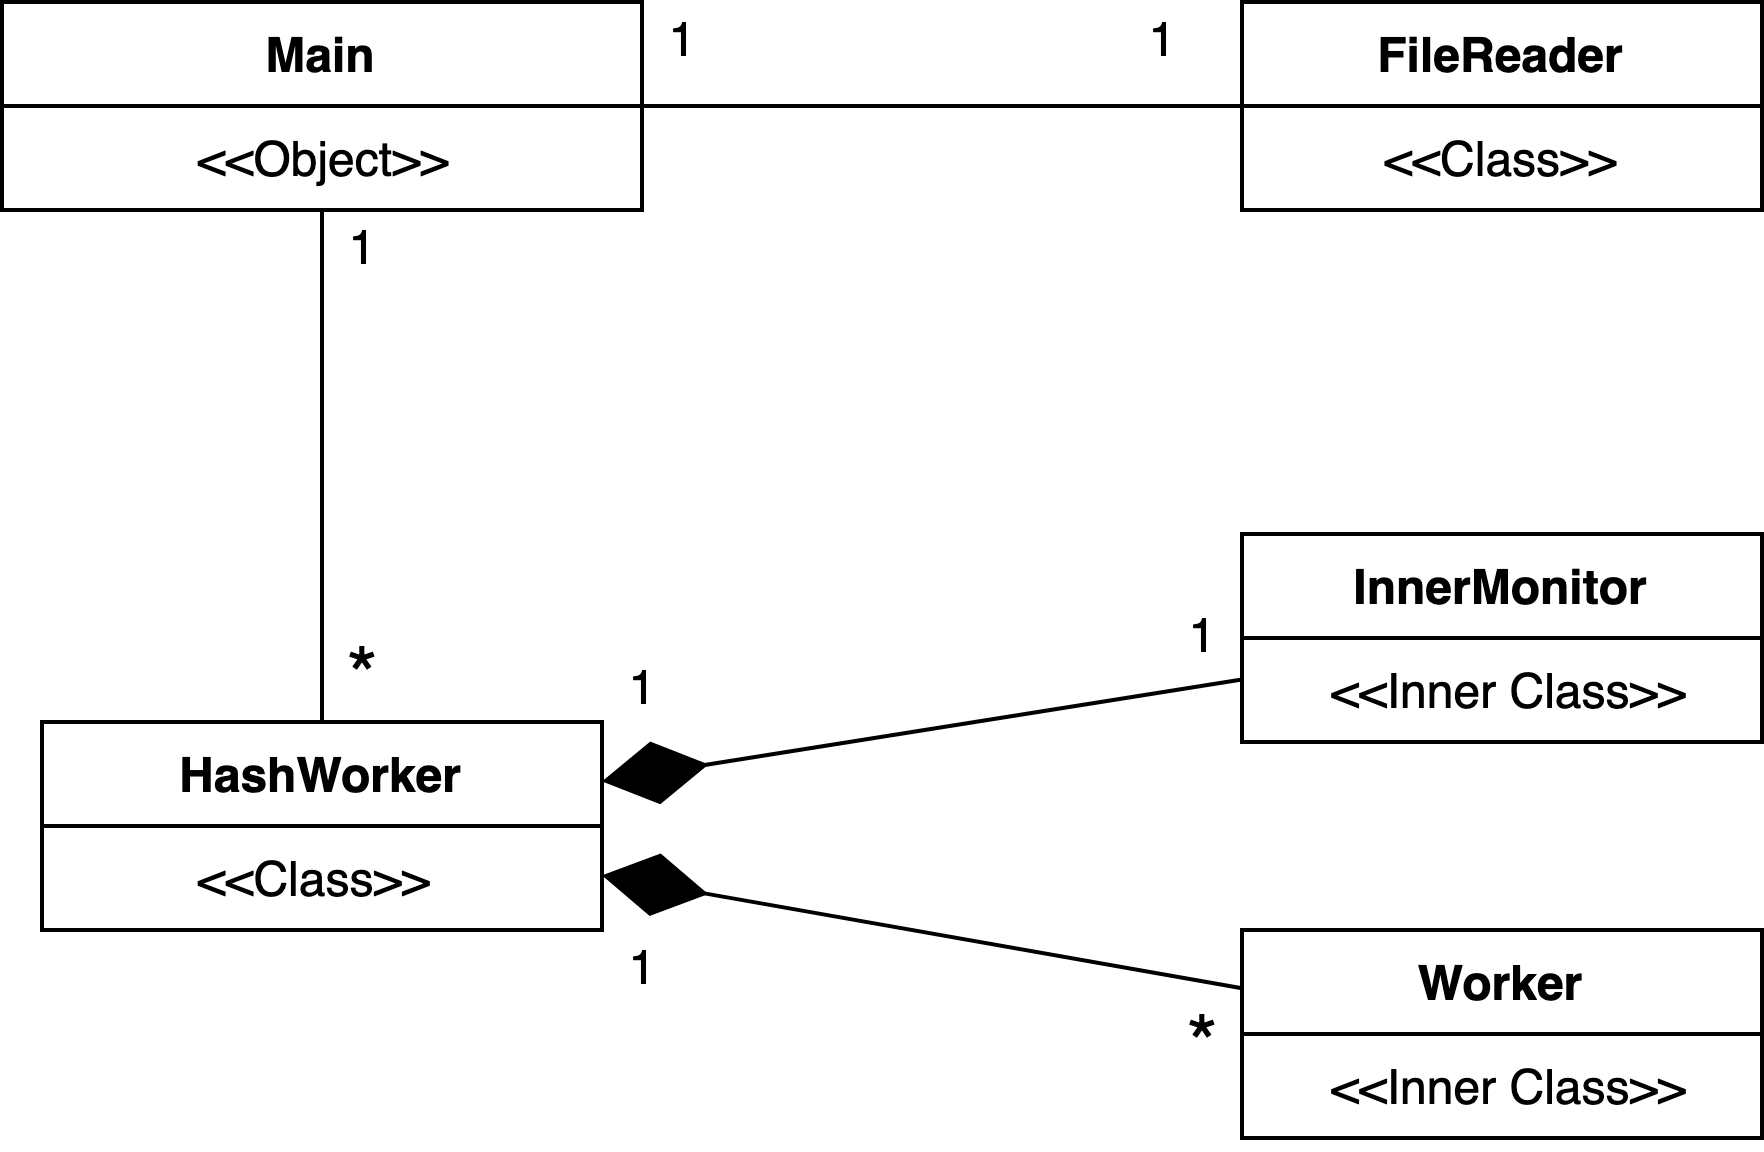
\includegraphics[scale=0.9]{chapters/implementation/figures/HashWorker_class_diagram.png}
    \caption{Illustration of the class structure used for computation offloading}
    \label{fig:HashWorker_class_diagram}
\end{figure}
Figure \ref{fig:HashWorker_class_diagram} shows the class structure. We have four classes and one object. We will now go through each of them and briefly explain what they do.


%Mention that since InternalMonitor has fields, getters and setters are automatically created at compile time, and since it is in a monitor, it is guaranteed that only one thread at a time can call those functions. 


\subsubsection{FileReader}
Below is the interface of class FileReader:
\begin{lstlisting}[language=emerald]
const FileReader <- class FileReader
  export op readFile[fileName: String] 
                            -> [res: Array.of[String]]
                            
  export function convertConfigToIntegers
                            [input: Array.of[String]] 
                          -> [res: Array.of[Integer]]
                            
  function stripLast[i: String] -> [o: String]
end FileReader
\end{lstlisting}
The operation \verb|readFile| will read the file with the path provided in parameter \verb|fileName|. For each line it reads, it will delete the last character with \verb|stripLast|, as it is a unwanted newline character. The function \verb|convertConfigToIntegers| is a function that converts an array of strings to an array of integers. This is needed because configs consists of lines of numbers, but they are read as strings.



\subsubsection{HashWorker}
Below is the interface of class HashWorker:
\begin{lstlisting}[language=emerald]
const HashWorker <- class HashWorker
                                [limitation: Integer]
  
  attached const workload %String

  attached const mon <- InnerMonitor.create

  attached const InnerMonitor 
                        <- monitor class InnerMonitor

  attached const Worker
                  <- class Worker[iterations: Integer]

  initially

  export op setLimitation[lim: Integer]
  
  export op doWork[iterations: Integer]

  export op collectTimeUsed -> [res: Time]
end HashWorker
\end{lstlisting}




\subsubsection{InternalMonitor}
Below is the whole class of InnerMontor:
\begin{lstlisting}[language=emerald]
attached const InnerMonitor 
                        <- monitor class InnerMonitor
  field waiting : Boolean <- true

  field timeTaken : Time <- nil
end InnerMonitor
\end{lstlisting}
As discussed in section \ref{emerald:field}, fields in Emerald automatically generates getters and setters. Since it is in a monitor class it is guaranteed that invoking them is mutual exclusive. In other words, the getters and setters that are automatically created within the class is safe to use in parallel. Variable \verb|timeTaken| is used to store the time used by the process in class \verb|Worker|. Variable \verb|waiting| is used to ensure that main does not collect \verb|timeTaken| before the worker is done.





\subsubsection{Worker}
The hashing algorithm we use is called \textit{Djb2}. Our implementation is a converted version from a C implementation found here\cite{noauthor_hash_nodate}.
\begin{lstlisting}[language=emerald]
function djb2Hash[str: String] -> [res: Integer]
  res <- 5381
  for i : Integer <- 0 while i < str.length 
                                    by i <- i + 1
    res <- res * 33 * str[i].ord
  end for
end djb2Hash
\end{lstlisting}
The algorithm takes a string, iterates over it and multiplies itself with 33 and the characters ordinal number. To make it even heavier, we convert the result to string, and then re-insert that into the hash function 10000 times. We see that as one iteration, as shown in figure \ref{fig:Hashing_algorithm_iteration}. In other words, the HashWorker will do what figure \ref{fig:Hashing_algorithm_iteration} shows, parameter \verb|iterations| number of times. Since we just throw out the result after each time, Emeralds garbage compiler will ensure that we have plenty of memory available. 
\begin{figure}[t]
    \centering
    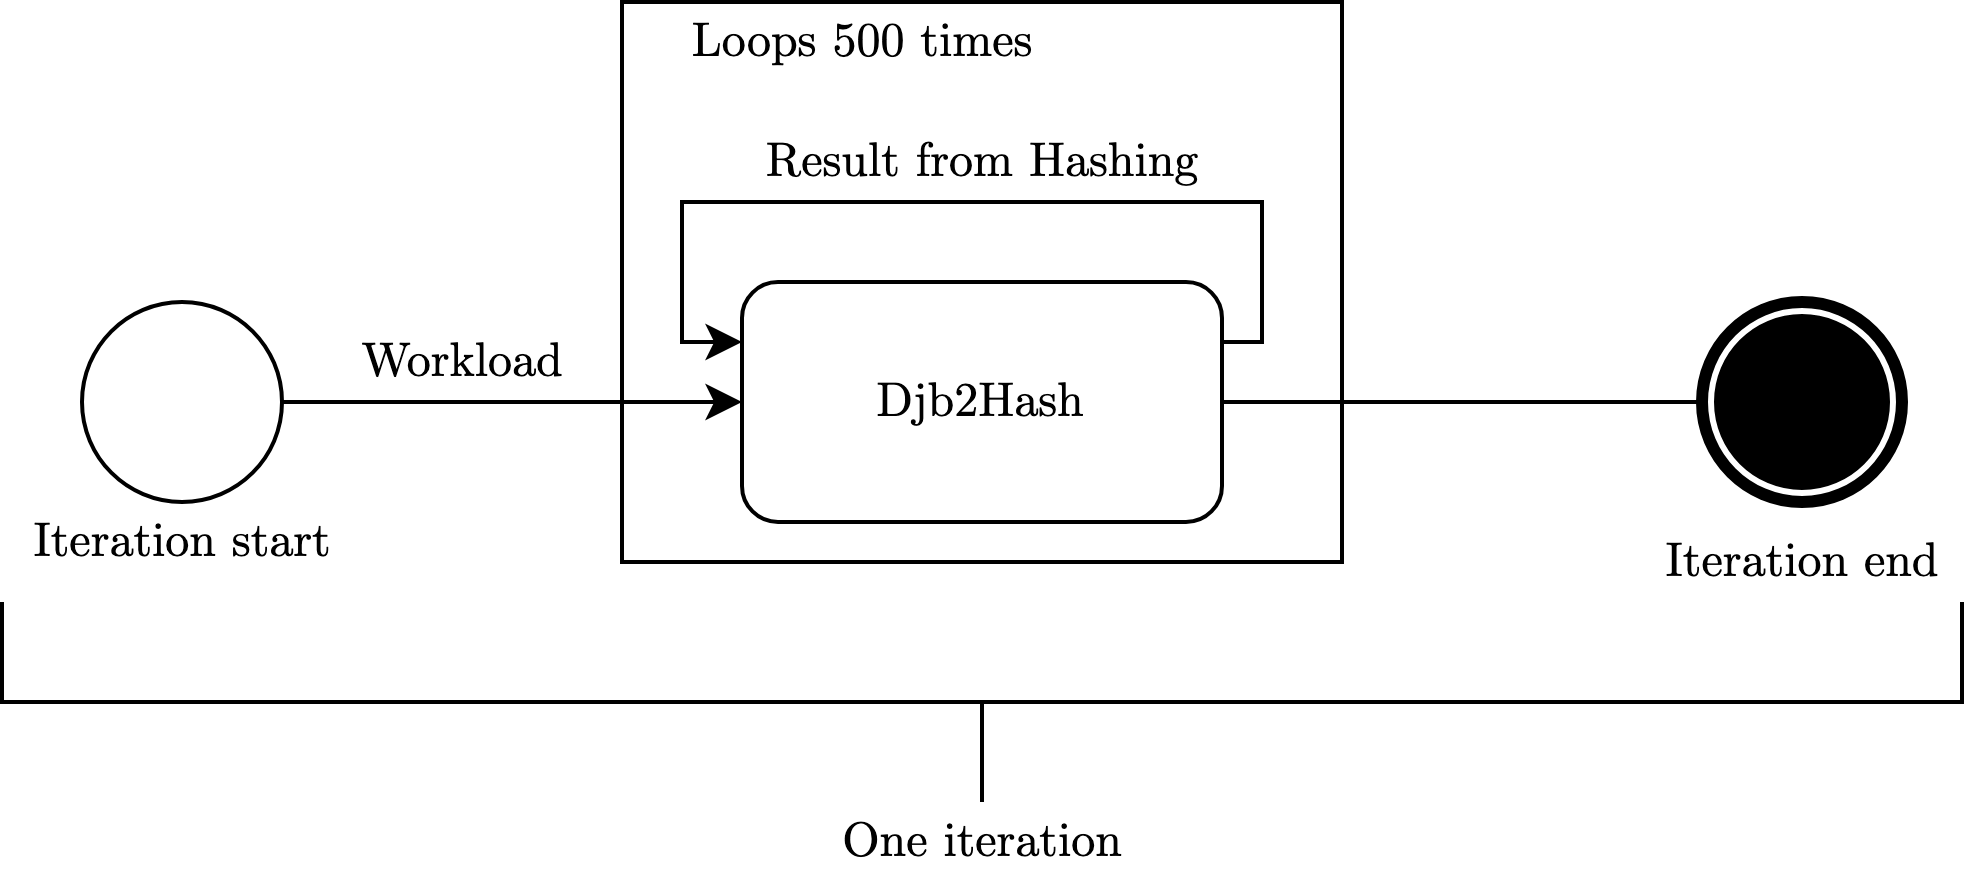
\includegraphics[scale=0.9]{chapters/implementation/figures/Iteration.png}
    \caption{Illustration of one iteration in the HashWorker}
    \label{fig:Hashing_algorithm_iteration}
\end{figure}




\subsubsection{Main}



\subsection{Simulating CPU restrictions}
To simulate CPU restrictions, we place a limitation on each HashWorker. This limitation is implemented as time delay. For each iteration a time delay is called. The amount of microseconds delayed is the \verb|limitation| parameter multiplied by 1000. 






\subsection{Storage offloading}












% -----------------------------------------------------------------------------------

\section{Multi-Access Edge Computing}
Figure TODO illustrates how three+ nodes will be set up. Blablabla.
TODO
% Vis de forskjellige måtene og ta storage offloading på


%\subsection{Limitation}
%Originally we wanted to use monitors. However when there is a case in Emerald where if you have to separate objects containing each of their own monitor with condition. Then when waiting on these separate conditions just exits the program when hitting the other condition!

